\documentclass[border=1pt]{standalone}
\usepackage{mathptmx}  % Times text and math
\usepackage{circuitikz}
\usetikzlibrary{arrows.meta}
\ctikzset{bipoles/length=0.75cm, transistors/scale=0.9,
  inductors/coils=4, current/distance=.5, bipoles/diode/height=.32,
  bipoles/diode/width=.26}
\begin{document}
\fontsize{8}{9.6}\selectfont
% single_loop: control diagram, 1 layout unit = 1 cm (ieee-double)
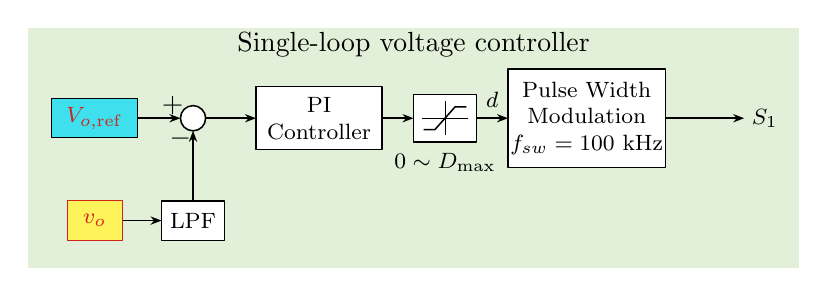
\begin{tikzpicture}[x=1cm, y=1cm, line width=0.55pt, line join=round]
% ---- regions (background) ----
\fill[fill={rgb,255:red,226;green,239;blue,217}] (-0.1,-1.9) rectangle (9.7,1.15);
\node[inner sep=0pt] at (4.8,0.94) {Single-loop voltage controller};
% ---- links ----
\draw[-{Stealth[length=0.14cm]}] (1.3,0) -- (1.84,0);
\draw[-{Stealth[length=0.14cm]}] (2.16,0) -- (2.8,0);
\draw[-{Stealth[length=0.14cm]}] (4.4,0) -- (4.8,0);
\draw[-{Stealth[length=0.14cm]}] (5.6,0) -- (6,0);
\draw[-{Stealth[length=0.14cm]}] (8,0) -- (9,0);
\draw[-{Stealth[length=0.14cm]}] (1.1,-1.3) -- (1.6,-1.3);
\draw[-{Stealth[length=0.14cm]}] (2,-1.05) -- (2,-0.16);
% ---- ref (tag) ----
\filldraw[fill={rgb,255:red,63;green,224;blue,238}, draw={rgb,255:red,0;green,0;blue,0}, line width=0.33pt] (0.2,-0.25) rectangle (1.3,0.25);
% ---- e1 (sum) ----
\draw[fill=white] (2,0) circle (0.16cm);
% ---- pi (block) ----
\draw[fill=white] (2.8,-0.4) rectangle (4.4,0.4);
% ---- lim (limiter) ----
\draw[fill=white] (4.8,-0.3) rectangle (5.6,0.3);
\draw[line width=0.275pt] (4.912,0) -- (5.488,0) (5.2,-0.216) -- (5.2,0.216);
\draw (4.928,-0.144) -- (5.072,-0.144) -- (5.328,0.144) -- (5.472,0.144);
% ---- pwm (block) ----
\draw[fill=white] (6,-0.625) rectangle (8,0.625);
% ---- vo (tag) ----
\filldraw[fill={rgb,255:red,255;green,243;blue,92}, draw={rgb,255:red,208;green,35;blue,28}, line width=0.33pt] (0.4,-1.55) rectangle (1.1,-1.05);
% ---- lpf (block) ----
\draw[fill=white] (1.6,-1.55) rectangle (2.4,-1.05);
% ---- signs ----
\node[inner sep=0pt] at (1.74,0.16) {$+$};
\node[inner sep=0pt] at (1.84,-0.26) {$-$};
% ---- text ----
\node[inner sep=0pt, align=center, font=\fontsize{8}{9.6}\selectfont, text={rgb,255:red,208;green,35;blue,28}] at (0.75,0) {$V_{o,\mathrm{ref}}$};
\node[inner sep=0pt, align=center, font=\fontsize{8}{9.6}\selectfont] at (3.6,0) {PI\\Controller};
\node[inner sep=0pt, align=center, font=\fontsize{8}{9.6}\selectfont] at (5.2,-0.56) {$0\sim D_{\max}$};
\node[inner sep=0pt, align=center, font=\fontsize{8}{9.6}\selectfont] at (7,0) {Pulse Width\\Modulation\\$f_{sw}=100$ kHz};
\node[inner sep=0pt, align=center, font=\fontsize{8}{9.6}\selectfont, text={rgb,255:red,208;green,35;blue,28}] at (0.75,-1.3) {$v_{o}$};
\node[inner sep=0pt, align=center, font=\fontsize{8}{9.6}\selectfont] at (2,-1.3) {LPF};
\node[inner sep=0pt, align=center, font=\fontsize{8}{9.6}\selectfont] at (5.8,0.23) {$d$};
\node[inner sep=0pt, align=center, font=\fontsize{8}{9.6}\selectfont] at (9.26,0) {$S_{1}$};
\end{tikzpicture}
\end{document}
